\section{Experiments}

\begin{figure}[ht]
\centering
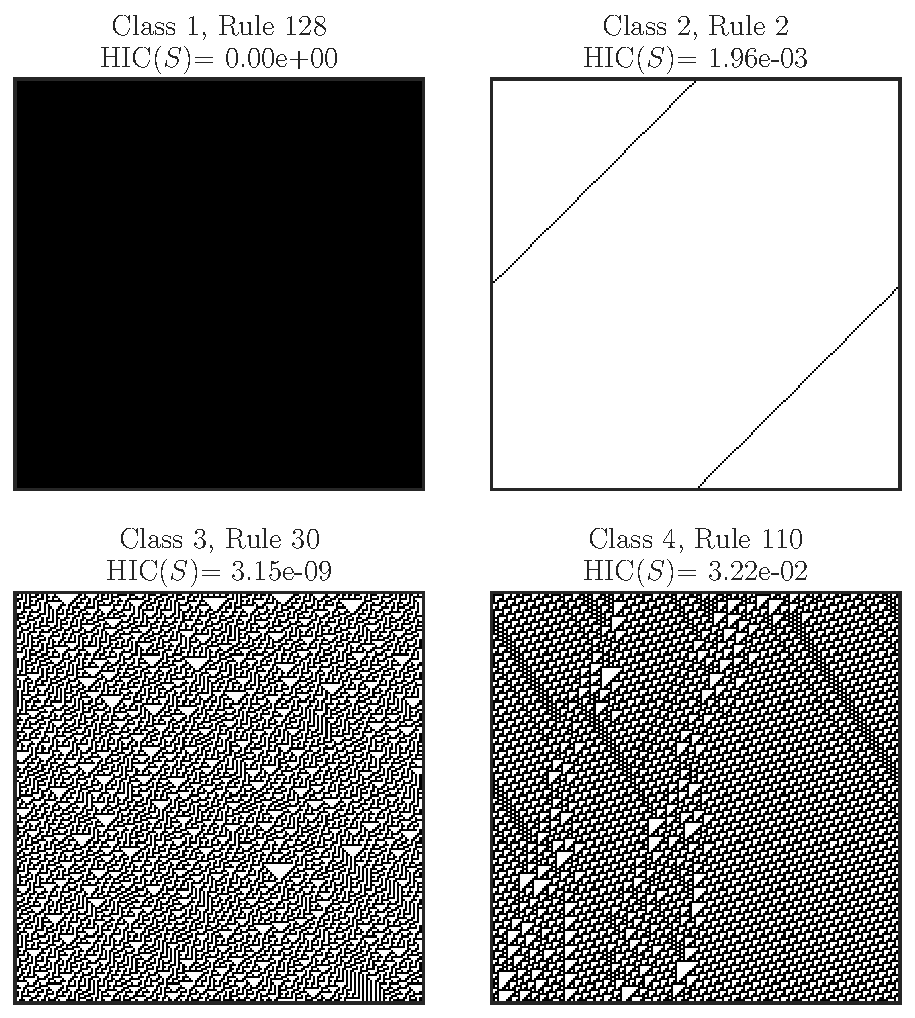
\includegraphics[width=0.7\textwidth]{figures/eca_images_and_hic}
\caption{TODO}
\label{fig:eca_images_and_hic}
\end{figure}

We examine HIC empirically using elementary cellular automata (ECA). Cells in
an ECA can take on one of two states. The update rule for a given state depends
on the state at the previous time step along with its two neighbors. Hence
there are $2^8 = 256$ possible ECAs. \citet{wolfram1983} proposed a four class
system to categorize ECA rules by their typical behavior. Class 1 ECAs converge
to a constant state, class 2 ECAs tend to exhibit periodic oscillations, class
3 ECAs display random-like behavior, and class 4 ECAs show complex behavior.
Complex behavior for an ECA is not well and determined mostly through
inspection. The typical manifestation are some high-level structure propagating
through time with some degree of apparant randomness interspersed between.
Despite the simplicity of the rules they yield astonishingly complex behavior.
Rule 110, for example, has been shown to be computationally
universal~\citep{cook2004universality}. We follow the Wolfram classification
given by~\citet[table 2]{martinez2013note} to classify all 256 ECA rules.

For each ECA we use a state size of $D$. The information in the initial state
requires at least $D/2$ updates to propagate accross the complete state space.
Hence we update the ECA for $2D$ time steps and discard the first $D$ time-step
states which provdes to provide an extra buffer for information in the initial
state to full propagate. Note that we use a circular update so that the cells
at the edges are influenced by neighbors at the opposite edge of the state.
Rules which propagate information unidirectionaly require the full buffer of
$D$ updates.

We use the remaining $D \times D$ cells to compute the HIC. At each level we
set $X^\ell$ and $Y^\ell$, the variables used to compute the mutual information
in equation~\ref{eq:mutual_information}, to be neighboring sequences each
consisting of $\ell$ cells. So for the first level ($\ell = 1$) $X$ and $Y$ are
single and consecutive cells, for $\ell = 2$ the variables are consecutive but
disjoint pairs of cells, and so on. We estimate the distributions $P(X^\ell)$
and $P(X^\ell \mid Y^\ell)$ used to compute the mutual information at each
level simply from counts over the states.

% TODO increase font size on figures
\begin{figure}[t]
\centering
\begin{subfigure}{0.45\textwidth}
  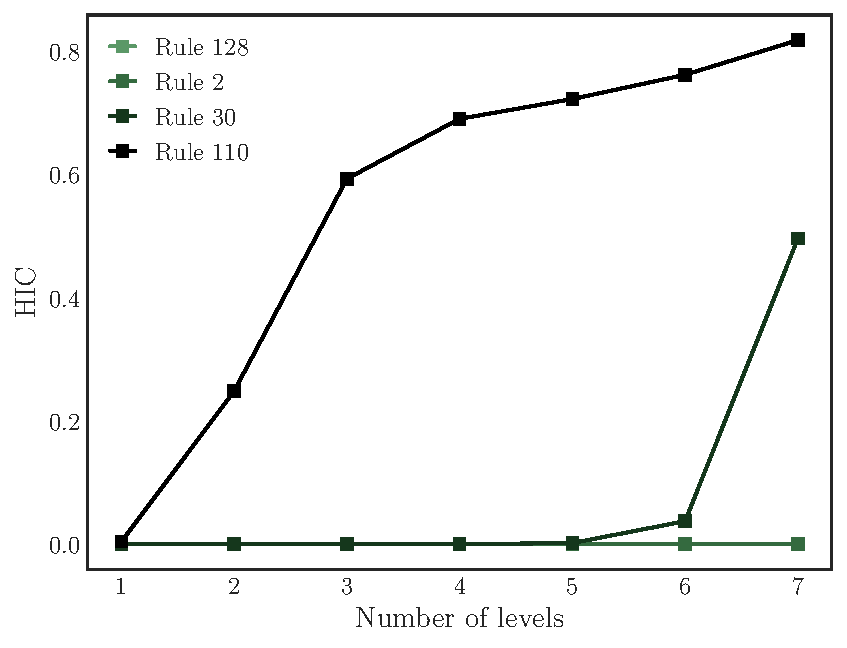
\includegraphics[width=1.0\textwidth]{figures/hic_vs_num_levels_size_200}
  \caption{State size $D = 200$}
  \label{fig:hic_levels_200}
\end{subfigure}
\begin{subfigure}{0.45\textwidth}
  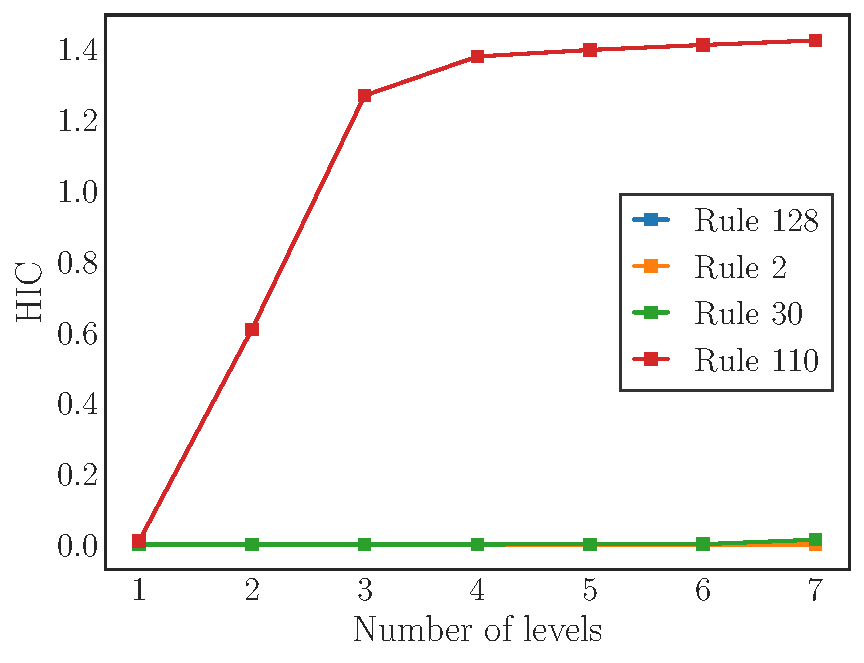
\includegraphics[width=1.0\textwidth]{figures/hic_vs_num_levels_size_500}
  \caption{State size $D = 500$}
  \label{fig:hic_levels_500}
\end{subfigure}
\caption{TODO}
\label{fig:hic_vs_levels}
\end{figure}

Figure~\ref{fig:eca_images_and_hic} shows a canonical ECA rule froom each
class: rule 128 is class 1, rule 2 is class 2, rule 30 is class 3, and rule 110
is class 4. For these simulations we use $D=200$ and initial state of all
inactive cells (zeros) with a single active cell (one) at the center. We
compute the HIC over $L=3$ levels. The HIC is given for each rule above the
corresponding image. Note that HIC correctly distinguishes rule 110 as being
the most complex ECA from the remainder which have HICs very close to zero.
Note in particular that the HIC of the class 3 ECA (rule 30) is even smaller
than the corresponding class 2 ECA (rule 2). In this case HIC peaks in-between
order and disorder, as desired.

With the same four rules, we observe the effect of the number of levels on the
HIC in figure~\ref{fig:hic_vs_levels}. Figure~\ref{fig:hic_levels_200} uses a
states size of $D=200$, and figure~\ref{fig:hic_levels_500} uses a state size
of $D=500$. In both figures, we see that the class 1 and 2 rules (the curves
overlap at zero) do not grow with an increase in the number of levels. The
class 4 rule grows but plateaus with the number of levels. We expect to see a
plateau once the size of the variables $X^\ell$ and $Y^\ell$ fully capture the
present structure, and so the mutual information should become constant. This
reflects the notion that complexity does not grow only via compositions of
order from order. Interposing disorder somewhere near the level of the largest
structures would result in further complexity growth.

The class 3 ECA is the only one which exhibits a qualitative difference between
the two figures. This is simply a statistical artefact which is useful to
elucidate. In the $D=200$ case, we do not have enough states to estimate the
mutual information at the highest level ($\ell = 7$) accurately. The mutual
information consists of two terms, the entropy of the single variable
$H(X^\ell)$ and the conditional entropy between the two variables $H(X^\ell
\mid Y^\ell)$. The entropy requires fewer samples to estimate accurately than
the conditional entropy. For example $X^7$ can take on $2^7$ possible values so
the pair $(X^7, Y^7)$ admits $2^14$ distinct values. As the gap becomes subject
to the influence of the number of samples we will the conditional entropy
shrinks with respect to the entropy artificially inlating the mutual
information. As we see this can be easily repairde by increasing $D$. However,
a parametric or otherwise more sample efficient model for $P(X)$ and $P(X \mid
Y)$ is an alternative that will likely scale more robustly with the number
of values of $X^\ell$.


